\bookchapter{第六十章：搭建開發環境——Xcode 同第一個項目}

\chapterintro{工欲善其事，必先利其器。呢一章我哋將個「廚房」搭好：裝好 Xcode、行通模擬器、建立人生第一個 iOS 項目，再將工程結構拆開睇個明白。裝好環境之後，你會第一次見到自己寫嘅代碼變成一個㩒得到嘅掣——呢個瞬間，好多人會記一世。}

\booksection{一、準備一部 Mac}

先講門檻：iOS 開發必須喺 macOS 上面進行。如果你冇 Mac，選擇有三：買一部（就算係二手 Mac mini 或者 MacBook Air 都夠用）、短期租雲 Mac、或者先讀第八篇《安卓開發實戰篇》（Windows 就得）。

\begin{center}
\begin{tabularx}{\linewidth}{|X|X|X|}
\hline
\textbf{配置項} & \textbf{最低要求} & \textbf{舒適線（推薦）} \tabularnewline
\hline
晶片 & Apple Silicon（M1 起） & M2 或更新 \tabularnewline
記憶體 & 8GB & 16GB \tabularnewline
磁碟 & 預留 40GB+（Xcode 本體好肥） & 256GB 起步 \tabularnewline
系統 & 最新 macOS & 保持自動更新 \tabularnewline
\hline
\end{tabularx}
\end{center}

\begin{center}\small\color{gray}Mac 開發機配置參考（2026 年 8 月）\end{center}

\begin{tcbinfo}{小貼士：冇 Mac 都可以先學語言}
iPad 上面免費嘅 Swift Playgrounds 可以學 Swift 語言基礎（唔使 Mac）；甚至 iPhone 上面都裝到。先將第 61 章嘅語言知識喺 Playgrounds 度玩熟，等攞到 Mac 之後就即刻起飛。磨刀唔誤砍柴工，講嘅就係呢樣。

\end{tcbinfo}

\booksection{二、安裝 Xcode}

Xcode 係蘋果官方嘅集成開發環境，免費。三步裝好：

\begin{enumerate}
  \item 喺 Mac 打開 App Store，搜「Xcode」，㩒安裝——留意佢有成幾個 GB，搵個網速好嘅時段；
  \item 裝完第一次啟動，同意協議、裝完組件（自動完成）；
  \item 選單 Xcode Settings Locations，確認 Command Line Tools 已經揀咗——命令行工具係好多腳本同第三方工具嘅前提。
\end{enumerate}

\begin{tcbwarn}{注意：版本同系統嘅「配對遊戲」}
新 Xcode 好多時都要求最新 macOS，舊 Mac 就會卡喺舊版本。上架 App Store 嗰陣，蘋果會要求用較新嘅 Xcode 構建（通常會畀一段寬限期）。所以系統更新唔好拖太耐——iOS 開發者係「追新版」最勤力嘅一群人。

\end{tcbwarn}

\booksection{三、建立你嘅第一個項目}

打開 Xcode Create New Project 揀 iOS App 模板，跟住填：

\begin{center}
\begin{tabularx}{\linewidth}{|X|X|X|}
\hline
\textbf{配置項} & \textbf{填乜嘢} & \textbf{說明} \tabularnewline
\hline
Product Name & MyFirstApp & 應用名 \tabularnewline
Team & 你嘅 Apple ID（免費） & 簽名用，個人賬號就得 \tabularnewline
Organization Identifier & com.example & 同 Product Name 拼埋組成包標識 \tabularnewline
Interface & SwiftUI & 本書主線框架 \tabularnewline
Language & Swift & 唔使解釋 \tabularnewline
\hline
\end{tabularx}
\end{center}

\begin{center}\small\color{gray}建立項目要填嘅五樣嘢\end{center}

㩒 Create 之後，Xcode 會生成一個可以直接行嘅項目。左上角揀一部模擬器（例如 iPhone 17），㩒 > 運行——幾秒之後，模擬器屏幕上面會出現一個寫住 “Hello, world!” 嘅窗口。你嘅第一個 iOS App 已經誕生咗喇。

\booksection{四、工程結構拆解：每個檔案係做乜嘢嘅}

左邊係工程導航器，新手只需要識呢幾個：

\begin{center}
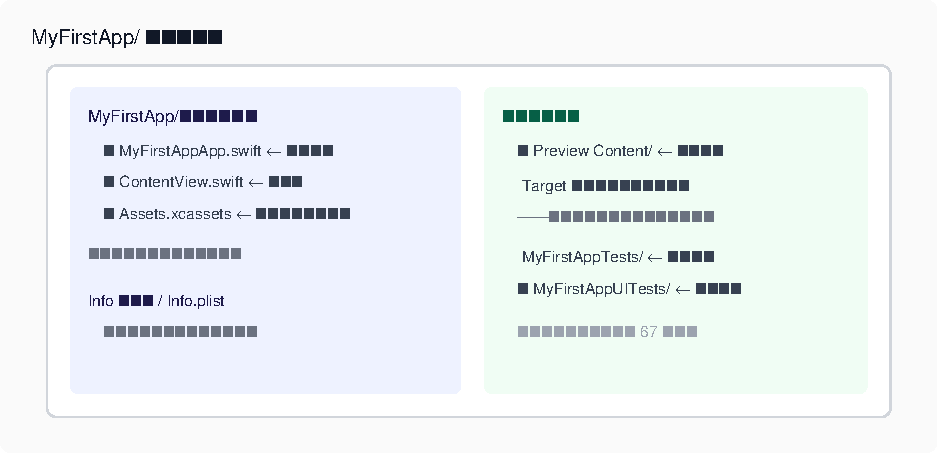
\includegraphics[width=0.92\linewidth]{figures/fig-di-liu-shi-zhang-1}
\\[2pt]\small 圖 2：新手必識嘅 Xcode 工程結構
\end{center}

\begin{itemize}
  \item MyFirstAppApp.swift：程式入口，喺 SwiftUI 入面佢只有幾行——「啟動，跟住顯示主界面」；
  \item ContentView.swift：主界面視圖，你而家見到嘅一切都在呢度；
  \item Assets.xcassets：資源倉庫——圖標、圖片、顏色都擺喺呢度；
  \item Target 設定：㩒左邊藍色工程圖標入去，版本號、最低 iOS 版本、簽名都在入面。App 顯示名、圖標都係喺呢度配置。
\end{itemize}

\booksection{五、真機除錯：將 App 裝入你嘅 iPhone}

\booksection{五、Xcode 效率技巧：新手嘅五個「快捷鍵外掛」}

用熟呢幾個，你會顯得「好專業」：

\begin{center}
\begin{tabularx}{\linewidth}{|X|X|X|}
\hline
\textbf{操作} & \textbf{快捷鍵} & \textbf{作用} \tabularnewline
\hline
運行 & CmdR & 編譯並且行起上嚟 \tabularnewline
打開/切換畫布預覽 & OptionCmd & 所見即所得嘅開關 \tabularnewline
格式化縮排 & CtrlI & 自動整理選中代碼嘅縮排 \tabularnewline
快速打開檔案 & CmdO & 輸入檔案名即刻開到（最常用！） \tabularnewline
註釋/取消註釋 & Cmd/ & 除錯嗰陣順手開關代碼 \tabularnewline
\hline
\end{tabularx}
\end{center}

\begin{center}\small\color{gray}Xcode 高頻快捷鍵（新手五件套）\end{center}

另外兩個隱藏福利：多開模擬器（同時行 iPhone 同 iPad 對比佈局）同代碼片段庫（將常用嘅幾行代碼拖入右邊 Snippets 面板，下次一鍵插入）——效率工具先用起上嚟，手感自然就上嚟喇。

\booksection{六、真機除錯：將 App 裝入你嘅 iPhone}

模擬器雖然好，但真機先係終點。用免費 Apple ID 都可以真機除錯：

\begin{enumerate}
  \item 數據線駁上 iPhone（或者同 Wi-Fi 無線除錯）；
  \item Xcode 頂部設備列表揀你部手機，第一次會提示登入 Apple ID 並且自動配置簽名；
  \item iPhone 上面 [設定] [一般] [VPN與設備管理] 信任你嘅開發者證書；
  \item 㩒 >，App 就裝入真機。
\end{enumerate}

\begin{tcbwarn}{注意：免費賬號嘅「七日限制」}
免費 Apple ID 簽名嘅 App 7 日之後會失效（重新運行一次就可以續期）。呢個係蘋果嘅防濫用機制，學習階段完全夠用；付費開發者賬號（99 美元/年）就冇呢個限制，第 67 章會詳細講。

\end{tcbwarn}

\booksection{七、小試牛刀 + 常見報錯急救}

\booksection{九、小試牛刀 + 常見報錯急救}

打開 ContentView.swift，將 Text(“Hello, world!”) 入面嘅字換成你個名，㩒 CmdR 重新運行——幾秒之後模擬器上面就會顯示你個名。恭喜，你完成咗第一次完整嘅「改代碼 編譯 安裝 運行」循環。

\begin{center}
\begin{tabularx}{\linewidth}{|X|X|X|}
\hline
\textbf{報錯現象} & \textbf{常見原因} & \textbf{解藥} \tabularnewline
\hline
Signing 報錯 & Team 冇揀、證書過期 & 喺 Target Signing 度剔返你嘅賬號；免費賬號重新行一次 \tabularnewline
模擬器黑屏/開唔到 & 映像損壞 & 選單 Device Erase All Content；或者刪咗佢重新加返模擬器 \tabularnewline
Xcode 下載慢/裝唔到 & App Store 網絡波動 & 轉個時段；或者去蘋果開發者網站下載 .xip 離線包 \tabularnewline
\hline
\end{tabularx}
\end{center}

\begin{center}\small\color{gray}新手環境報錯急救表\end{center}

\begin{tcbpractice}{嚟動手：完成你嘅「開發儀式感」清單}
(1) 裝好 Xcode 並且行通模擬器；(2) 用真機行一次自己嘅 App 並且截圖留念；(3) 將 Hello 文字改成你個名；(4) 去 Target 設定度將 App 顯示名改成「我嘅第一個App」。做完呢四步，你已經係一個有作品嘅人喇。

\end{tcbpractice}

\begin{tcbsummary}{本章小結}
\begin{itemize}
  \item 硬門檻：Mac + Xcode；冇 Mac 就先用 iPad 上面嘅 Swift Playgrounds 學語言
  \item Xcode 由 App Store 裝；新版本要求新系統，更新唔好拖
  \item 新建立項目五要素：名、Team、組織標識、SwiftUI、Swift
  \item 工程口訣：代碼都在 MyFirstApp/ 目錄；Target 設定管版本同簽名
  \item 免費 Apple ID 真機除錯有 7 日簽名限制；付費賬號冇呢個限制
  \item 開發日常 = 改代碼 CmdR 睇效果，循環不息
\end{itemize}

\end{tcbsummary}
